\chapter{Dynamic Modeling of Water-Skipping Motion}

\label{dynamic}

\section{Overview of Water-Skipping Process}

A hop is a single exchange of energy with the water surface.  The vehicle
arrives spinning and descending; it leaves spinning more slowly and rising.
Everything that makes the manoeuvre possible happens in the few tens of
milliseconds in between, and this chapter is concerned with what governs that
interval.

The mechanism rests on the vehicle's rotation.  Four hydrofoils are carried on
the airframe and turn with it, so that each sweeps a circular path at a
tangential speed $\omega r$ set by the spin rate and its radius.  That speed is
an order of magnitude larger than the vehicle's descent speed, which means the
foils meet the water almost edge-on, travelling far faster sideways than
downward.  Inclined at a fixed angle $\beta$, each foil therefore acts as a
lifting surface driven by the spin rather than by the fall.

What makes this worth doing is the density of the fluid.  The same foils sweep
through air during flight, but water is roughly three orders of magnitude
denser, so a foil that produces a negligible force in air produces a large one
the instant it is immersed.  The vehicle thus carries surfaces that cost little
in flight yet can arrest its descent on contact.

The contact itself proceeds in two competing directions.  The foils generate a
vertical force that decelerates and then reverses the vehicle, and
simultaneously a resisting torque that drains the spin which produces that
force.  A hop succeeds when the vertical impulse is large enough to return the
vehicle to the air before the spin has decayed too far to keep it controllable
once there.  The model developed in this chapter quantifies both effects: the
quasi-steady hydrodynamics of a single foil section
(Section~\ref{sec:quasi_steady}), their integration along the span
(Section~\ref{sec:blade_element}), and the coupled vertical and rotational
motion that results (Section~\ref{sec:vertical_rotational}).

\paragraph{Scope and assumptions.}
The treatment is deliberately economical.  Forces are taken as quasi-steady,
so that each instant is evaluated as if the flow were in equilibrium; the
foils are modelled as flat plates, with the separated-flow coefficients that
follow; only the submerged portion of a foil is assumed to generate force, and
the water surface is treated as flat and undisturbed, so that the wetted extent
of a foil is fixed by its geometric depth alone.  Air loads during the contact
are neglected beside the hydrodynamic ones.  These assumptions make the problem
tractable and expose the parameters that matter, at the cost of quantitative
fidelity where the free surface deforms appreciably; Chapter~\ref{chapter:paperthree}
compares the resulting predictions with flight measurements and returns to this
point.

\section{Quasi-Steady Blade-Element Model}
\label{sec:quasi_steady}

Because the density of water exceeds that of air by three orders of magnitude,
the force generated by the submerged portion of a hydrofoil dominates the
motion of the vehicle during contact, and only that force is retained here.

The foil is not a single lifting surface with one velocity.  It rotates with
the airframe, so its local speed varies along the span, and it is therefore
treated by the blade-element method: the foil is divided into elements of
radial width $dr$, each evaluated as a two-dimensional section under
quasi-steady conditions, and the element forces are integrated along the span.
The quasi-steady hydrodynamics are introduced directly at the element level
below, since that is the only level at which they are applied.

\paragraph{Element kinematics.}
Figure~\ref{fig:model_definitions}(B) shows the foil in plan view.  It occupies
an annular band of the swept disk, beginning at the root radius
$r_{\mathrm{in}}$ fixed by the motor-mount circle and extending to the tip
radius $r_{\mathrm{tip}}$; its radial span is $r_{\mathrm{tip}}-r_{\mathrm{in}}$,
and no lifting surface occupies $r<r_{\mathrm{in}}$.

An element at radius $r$ meets the water with two velocity components: a
horizontal component due to the rotation of the vehicle, and a vertical
component due to its descent.  The horizontal component is the local
tangential speed
%
\begin{equation}
    v_x(r) = \omega r ,
    \label{eq:blade_tangential_velocity}
\end{equation}
%
which varies along the span, so every quantity derived from it is a function of
$r$.  The vertical component is the descent rate $\dot{z}$, common to the whole
vehicle.  The resultant speed of the element relative to the water is therefore
%
\begin{equation}
    v(r) = \sqrt{(\omega r)^2 + \dot{z}^{\,2}} .
    \label{eq:blade_resultant_velocity}
\end{equation}
%
The angle between this resultant and the horizontal is the inflow angle
%
\begin{equation}
    \gamma(r) = \tan^{-1}\!\left(\frac{-\dot{z}}{\omega r}\right),
    \label{eq:blade_gamma}
\end{equation}
%
where $\dot{z}<0$ during the descent, so $-\dot{z}$ is the downward speed.  The
foil is mounted at a fixed inclination $\beta$ to the horizontal, so the local
angle of attack combines that inclination with the inflow direction
(Figure~\ref{fig:model_definitions}(A)):
%
\begin{equation}
    \alpha(r) = \beta + \gamma(r) .
    \label{eq:blade_alpha}
\end{equation}
%
Here $\omega$ is the angular velocity of the vehicle and $\dot{z}$ its vertical
velocity.  Since $\gamma$ depends on $r$, so does $\alpha$: the angle of attack
is largest at the root, where the tangential speed is lowest and the inflow
steepest, and approaches $\beta$ at the tip.

\paragraph{Element forces.}
Under the quasi-steady assumption each element is evaluated as if the flow
around it were in equilibrium, so the standard sectional expressions apply with
the local speed and angle of attack of \eqref{eq:blade_resultant_velocity}
and~\eqref{eq:blade_alpha}.  For a flat plate in separated flow the sectional
coefficients are
%
\begin{equation}
    C_L(\alpha) = 2 \sin{\alpha}\cos{\alpha},
    \qquad
    C_D(\alpha) = 2 \sin^2{\alpha},
    \label{eq:flat_plate_coeffs}
\end{equation}
%
which hold for a thin plate at large angle of attack, where the flow separates
at both edges and the resultant force acts normal to the
plate~\cite{bocquet2003physics,truscott2014water}.

Because the hydrofoil is a thin slanted plate, the portion submerged at penetration depth $z$ extends a length $z/\sin{\beta}$ along the chordwise (slant) direction. This wetted length grows with depth only until the plate is fully wetted, which occurs at the depth $h^{*} = c\sin{\beta}$, where $c$ is the physical chord of the foil; at greater depths the wetted length is bounded by the chord itself. The submerged chord is therefore

\begin{equation}
    c_{\mathrm{sub}} = \min\!\left(\frac{z}{\sin{\beta}},\; c\right),
    \label{eq:submerged_chord}
\end{equation}
and is the same for every blade element at a given instant. The submerged area of a blade element of radial length $dr$ is then

\begin{equation}
    dS = c_{\mathrm{sub}}\,dr .
    \label{eq:blade_area}
\end{equation}

Based on the quasi-steady assumption, the differential lift and drag generated by this blade element are

\begin{equation}
    dF_L = \frac{1}{2}\rho C_L(\alpha) v^2(r)\,c_{\mathrm{sub}}\,dr ,
    \label{eq:differential_lift}
\end{equation}

\begin{equation}
    dF_D = \frac{1}{2}\rho C_D(\alpha) v^2(r)\,c_{\mathrm{sub}}\,dr ,
    \label{eq:differential_drag}
\end{equation}
where $\rho$ is the density of water, and $C_L(\alpha)$ and $C_D(\alpha)$ are the lift and drag coefficients.

The differential vertical thrust and horizontal resistance force are obtained by decomposing the lift and drag forces:

\begin{equation}
    dT = dF_L \cos{\gamma(r)} + dF_D \sin{\gamma(r)} ,
    \label{eq:differential_thrust}
\end{equation}

\begin{equation}
    dF_R = dF_D \cos{\gamma(r)} - dF_L \sin{\gamma(r)} .
    \label{eq:differential_resistance}
\end{equation}

The horizontal resistance force produces a resisting torque about the rotational center:

\begin{equation}
    dQ = r\,dF_R
    =
    r\left(dF_D \cos{\gamma(r)} - dF_L \sin{\gamma(r)}\right).
    \label{eq:differential_torque}
\end{equation}


\section{Vertical Motion and Rotational Dynamics}
\label{sec:vertical_rotational}

The total vertical thrust and resisting torque generated by one hydrofoil are obtained by integrating the blade elements along the radial direction, over the span the foil actually occupies: from the root radius $r_{\mathrm{in}}$ to the tip radius $r_{\mathrm{tip}}$. The lower limit is consequential. Because the element force grows as $(\omega r)^2$, extending the integral inward to the axis would not add a small correction but would credit the vehicle with a stretch of foil it does not carry. The chord $c$ enters the model only as the saturation limit of the submerged chord $c_{\mathrm{sub}}$ of~\eqref{eq:submerged_chord}: in the shallow phase of the contact the wetted length is set by the penetration depth alone, while in the deeper phase it is bounded by the physical extent of the foil.

Substituting the differential lift and drag into the force decomposition, the total vertical thrust generated by one hydrofoil is

\begin{equation}
    T_{\mathrm{foil}}
    =
    \int_{r_{\mathrm{in}}}^{r_{\mathrm{tip}}}
    \frac{1}{2}\rho c_{\mathrm{sub}} v^2(r)
    \left[
    C_L(\alpha(r))\cos{\gamma(r)}
    +
    C_D(\alpha(r))\sin{\gamma(r)}
    \right] dr .
    \label{eq:total_thrust_c}
\end{equation}

Similarly, the resisting torque generated by one hydrofoil is

\begin{equation}
    Q_{\mathrm{foil}}
    =
    \int_{r_{\mathrm{in}}}^{r_{\mathrm{tip}}}
    \frac{1}{2}\rho c_{\mathrm{sub}} r v^2(r)
    \left[
    C_D(\alpha(r))\cos{\gamma(r)}
    -
    C_L(\alpha(r))\sin{\gamma(r)}
    \right] dr .
    \label{eq:total_torque_c}
\end{equation}

If the vehicle has $N$ identical hydrofoils that contact the water under the same condition, the total vertical thrust and resisting torque are approximated as

\begin{equation}
    T = N T_{\mathrm{foil}},
    \label{eq:total_vehicle_thrust}
\end{equation}

\begin{equation}
    Q = N Q_{\mathrm{foil}}.
    \label{eq:total_vehicle_torque}
\end{equation}

In practice, $N$ represents the number of effective hydrofoils in contact with the water at a given time step.

Combining the above equations, the total vertical thrust and resisting torque can be summarized as nonlinear functions of the vehicle states and hydrofoil design parameters:

\begin{align}
    T &= T\left(
        z,\dot{z},\omega,r_{\mathrm{in}},r_{\mathrm{tip}},c,\beta,N,\rho
    \right),
    \label{eq:T_function} \\[2pt]
    Q &= Q\left(
        z,\dot{z},\omega,r_{\mathrm{in}},r_{\mathrm{tip}},c,\beta,N,\rho
    \right).
    \label{eq:Q_function}
\end{align}

The vertical and rotational dynamics of the vehicle during water impact are then written as

\begin{align}
    m\ddot{z} &= \phantom{-}T\left(
        z,\dot{z},\omega,r_{\mathrm{in}},r_{\mathrm{tip}},c,\beta,N,\rho
    \right) - mg,
    \label{eq:vertical_dynamics_function} \\[2pt]
    I\dot{\omega} &= -Q\left(
        z,\dot{z},\omega,r_{\mathrm{in}},r_{\mathrm{tip}},c,\beta,N,\rho
    \right).
    \label{eq:rotational_dynamics_function}
\end{align}

In this formulation the hydrofoil geometry enters through two parameters: the root and tip radii $r_{\mathrm{in}}$ and $r_{\mathrm{tip}}$, which set the radial integration range $r_{\mathrm{in}} \le r \le r_{\mathrm{tip}}$ ($r_{\mathrm{in}}$ being fixed by the airframe and $r_{\mathrm{tip}}$ taken as the design variable), and the chord $c$, which bounds the chordwise wetting. The submerged chord $c_{\mathrm{sub}} = \min(z/\sin{\beta},\,c)$ grows with the penetration depth in the shallow phase of the contact and saturates at the physical chord once the plate is fully wetted, at depths beyond $h^{*} = c\sin{\beta}$.
\section{Simulation}
\label{sec:simulation}

The coupled vertical and rotational dynamics of~\eqref{eq:vertical_dynamics_function} and~\eqref{eq:rotational_dynamics_function} are integrated numerically through a single water contact. Starting from the instant the foils touch the surface, the state $(z,\dot{z},\omega)$ is advanced with a fixed-step semi-implicit Euler scheme until the foils leave the water, that is, until $z$ returns to the surface with an upward velocity. For a given entry condition (entry spin $\omega_0$ and downward entry velocity $\dot{z}_0$) and foil geometry (root radius $r_{\mathrm{in}}$, tip radius $r_{\mathrm{tip}}$ and inclination $\beta$), the simulation returns the two quantities that characterise the hop: the exit spin $\omega_{\mathrm{exit}}$ and the exit vertical velocity $\dot{z}_{\mathrm{exit}}$.


\paragraph{Anatomy of a hop.}
Figure~\ref{fig:hop_time_history} overlays nine simulated contacts at the as-built tip radius of $145~\mathrm{mm}$, combining three foil inclinations ($\beta = 10^\circ, 28^\circ, 45^\circ$) with three entry speeds ($\dot{z}_0 = -1, -2, -3~\mathrm{m\,s^{-1}}$), all entering at the measured spin of $\omega_0 = 8000~\mathrm{deg\,s^{-1}}$. Solid curves are the vertical velocity $\dot{z}(t)$ on the left axis, dashed curves the spin $\omega(t)$ on the right, and filled circles mark the instant the foils leave the water.

Every case in this set ejects. The descent is arrested and reversed within $3.7$--$4.9~\mathrm{ms}$, and the vehicle leaves the surface climbing at $0.8$--$2.3~\mathrm{m\,s^{-1}}$ while retaining between $79\%$ and $99\%$ of its entry spin. The ordering is systematic: within each group of three, a faster entry produces a larger hop, and across the groups a steeper foil produces a longer contact and a heavier spin loss. The shallow $\beta = 10^\circ$ contacts give up almost no spin at all, while the steep $\beta = 45^\circ$ contact at the fastest entry surrenders a fifth of it.

Two features of the traces carry the physics. First, the reversal is not symmetric: each velocity curve turns sharply upward and then flattens as it approaches the surface, because the spin that generates the lift is itself being consumed. Second, the spin curves fall monotonically and never recover during the contact; whatever is spent is spent for good, and must be restored by the rotors during the flight that follows. The water contact is therefore not a conservative bounce. Its role is to \emph{reverse the vertical velocity and return the vehicle to the air with enough spin left to be controllable}, and the balance between those two demands is what the design study below quantifies.

\begin{figure}[t]
    \centering
    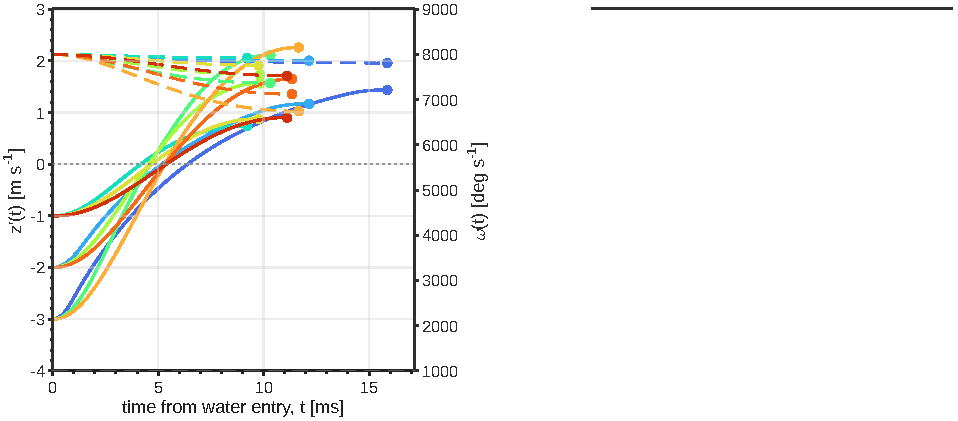
\includegraphics[width=\linewidth]{Assets/ch2fig1_hop_trajectories.pdf}
    \caption{Simulated time histories of nine water contacts at the as-built tip radius $r_{\mathrm{tip}} = 145~\mathrm{mm}$ and root radius $r_{\mathrm{in}} = 75~\mathrm{mm}$, combining three inclinations ($\beta = 10^\circ, 28^\circ, 45^\circ$) with three entry speeds ($\dot{z}_0 = -1, -2, -3~\mathrm{m\,s^{-1}}$), all entering at $\omega_0 = 8000~\mathrm{deg\,s^{-1}}$. Solid curves: vertical velocity $\dot{z}$ (left axis). Dashed curves: spin $\omega$ (right axis). Filled circles mark water exit. All nine contacts eject; steeper inclination and faster entry both lengthen the contact and increase the spin surrendered to the water.}
    \label{fig:hop_time_history}
\end{figure}

\paragraph{Design space and the hop--spin trade-off.}
Evaluating the model across the space spanned by the inclination $\beta$, the tip radius $r_{\mathrm{tip}}$, and the entry velocity $\dot{z}_0$ shows how the two hop metrics respond to the design. Figure~\ref{fig:design_space_maps} plots every simulated design as a point in this space, coloured by the exit vertical velocity $\dot{z}_{\mathrm{exit}}$ (left, the hop) and by the exit spin $\omega_{\mathrm{exit}}$ (right, the spin retained for the flight that follows). Across the space the hop ranges from $0.36$ to $3.17~\mathrm{m\,s^{-1}}$ and the retained spin from $4159$ to $7980~\mathrm{deg\,s^{-1}}$, between $52\%$ and essentially all of the entry spin.

The two panels are organised by different variables, and the contrast is the substance of the figure. The hop follows the entry velocity above all: the left panel is layered almost entirely along the $\dot{z}_0$ axis, and holding the geometry fixed while varying the entry speed alone moves $\dot{z}_{\mathrm{exit}}$ by $85\%$ of its range. The inclination $\beta$ is the second lever, worth a further $37\%$; a steeper foil presents more of its area to the flow and turns more of the sweep into vertical impulse. The tip radius is nearly inert by comparison, changing the hop by only about $4\%$ across a two-fold change in radius, because at the sweep speeds considered here the foils already generate far more force than is needed to reverse the descent, and the contact ends before the extra radius can express itself.

The retained spin behaves in the opposite sense. It is largest, close to the full entry value, where the foils do least work: shallow inclination and gentle entry. It falls steadily as either the inclination steepens or the entry speed rises, reaching $52\%$ at the most heavily loaded corner of the space. The two objectives therefore oppose one another: within this model the largest hop, $3.17~\mathrm{m\,s^{-1}}$, occurs at $\beta = 42^{\circ}$ and the fastest entry considered, and costs a quarter of the spin, while the design that retains all of its spin delivers a hop of only $0.36~\mathrm{m\,s^{-1}}$.

This is the compromise that sizes the vehicle: take as much hop as can be had while leaving enough spin for the vehicle to remain controllable on exit. It also indicates where design effort is repaid. The inclination and the conditions of entry govern the outcome, whereas the radial extent of the foil, once large enough, does not, so the foil may be sized by structural and packaging considerations without penalising the hop. The geometry selected on this basis is described in Chapter~\ref{chapter:paperone}.

\begin{figure}[t]
    \centering
    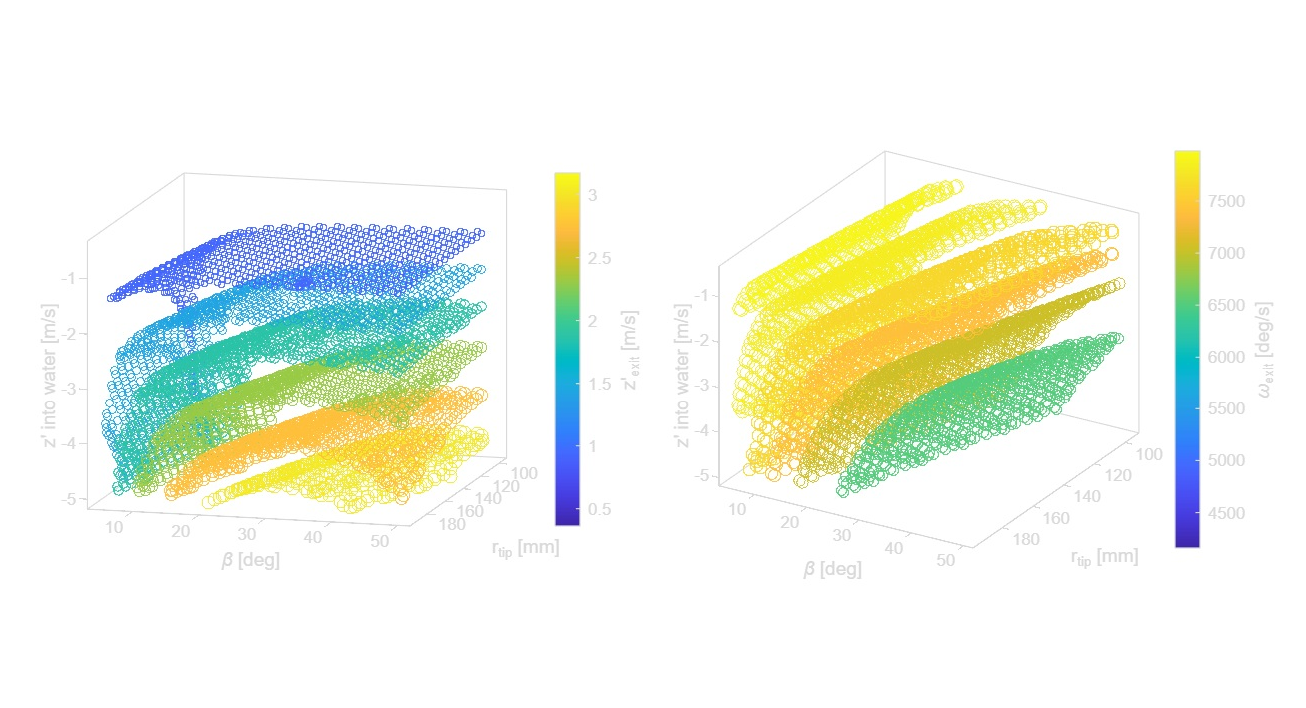
\includegraphics[width=\linewidth]{Assets/ch2fig2_design_space.pdf}
    \caption{Hop performance over the design space $(\beta,\ r_{\mathrm{tip}},\ \dot{z}_0)$, evaluated at the as-built root radius $r_{\mathrm{in}} = 75~\mathrm{mm}$ and entry spin $\omega_0 = 8000~\mathrm{deg\,s^{-1}}$. Each point lies on an iso-value surface of the response, coloured by the exit vertical velocity $\dot{z}_{\mathrm{exit}}$ (left, the hop) and by the exit spin $\omega_{\mathrm{exit}}$ (right, the retained spin). The two responses are organised by different variables: the hop is layered along the entry velocity and, secondarily, the inclination, while the retained spin falls wherever the foils are most heavily loaded. Both are nearly independent of the tip radius over the range shown.}
    \label{fig:design_space_maps}
\end{figure}